\subsubsection{Example}

    \begin{itemize}[noitemsep,topsep=0pt]
      \item Starting position: (-39.0, 68.0, 112.0)
      \item End position: (-2.0, 7.0, 7.0) 
      \item Euclidean distance from the object: 10.099504938362077
      \item Object can be seen: True
      \item Success: True
      \item Object type: fire
      
    \end{itemize}
    

    \begin{center}
    \includegraphics[width=0.7\linewidth]{images/GPT4o-CityNew-FS2/31.pdf}
    \end{center}
    

    \begin{center}
    \includegraphics[width=0.7\linewidth]{images/GPT4o-CityNew-FS2/31_sit_awareness.pdf}
    \end{center}
    

    \begin{drama}
    \Character{Benchmark}{re}
    \Character{GPT-4o}{gpt}
    
\respeaks: \( < \)Context\( > \)
    You are in command of a UAV, tasked with finding fire.
\( < \)/Context\( > \) \texttt{(REST OF THE PROMPT)}
\respeaks: The object you're looking for is similar to this. This is NOT the drone's current view.
\StageDir{\re{} presents \gpt{} with a relevant image}

    \begin{center}
    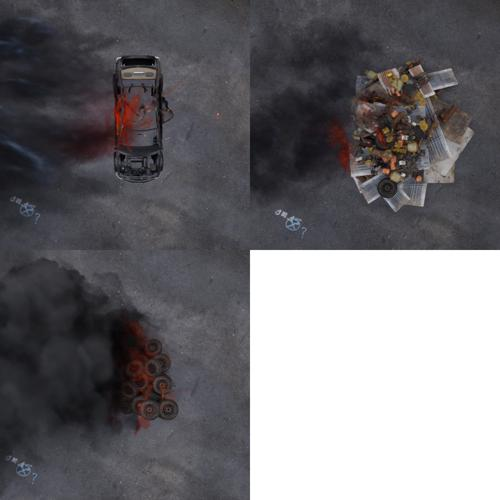
\includegraphics[width=0.5\linewidth]{images/GPT4o-CityNew-FS2/31_0.jpg}
    \end{center}
    
\respeaks: Your current altitude is 112 meters above ground level.
\StageDir{\re{} presents \gpt{} with a relevant image}

    \begin{center}
    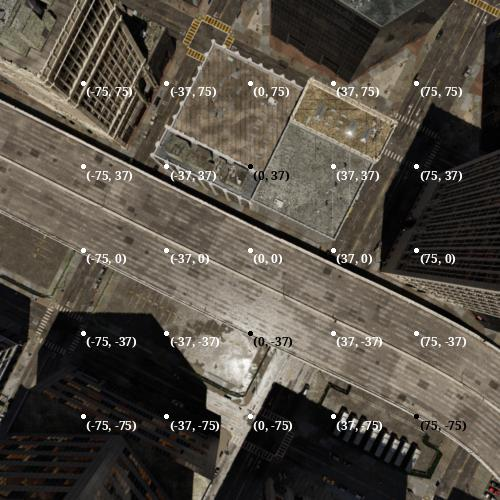
\includegraphics[width=0.5\linewidth]{images/GPT4o-CityNew-FS2/31_1.jpg}
    \end{center}
    
\gptspeaks: \( < \)Reasoning\( > \)Based on the image, I will start by moving towards the open area slightly to the north and to the right to get a better view. I'll also descend to get closer to the ground.\( < \)/Reasoning\( > \)
\( < \)Action\( > \)(37, 37, -40)\( < \)/Action\( > \)
\respeaks: Your current altitude is 72 meters above ground level.
\StageDir{\re{} presents \gpt{} with a relevant image}

    \begin{center}
    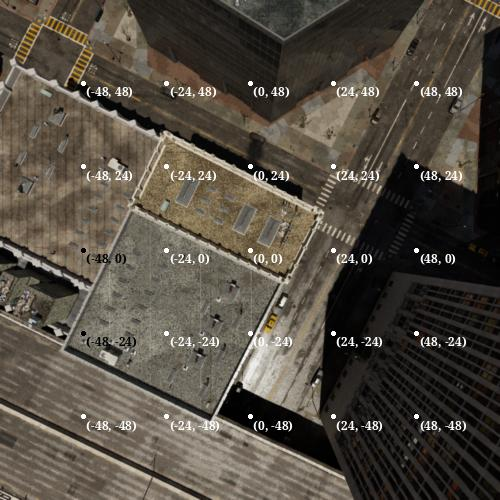
\includegraphics[width=0.5\linewidth]{images/GPT4o-CityNew-FS2/31_2.jpg}
    \end{center}
    
\gptspeaks: \( < \)Reasoning\( > \)I will continue moving towards the center of the open area, which might provide a better vantage point. I'll also descend further to improve visibility of potential fire sources.\( < \)/Reasoning\( > \)
\( < \)Action\( > \)(0, 24, -40)\( < \)/Action\( > \)
\respeaks: Your current altitude is 32 meters above ground level.
\StageDir{\re{} presents \gpt{} with a relevant image}

    \begin{center}
    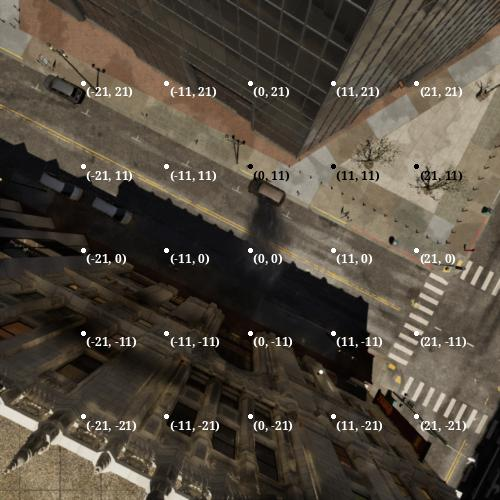
\includegraphics[width=0.5\linewidth]{images/GPT4o-CityNew-FS2/31_3.jpg}
    \end{center}
    
\gptspeaks: \( < \)Reasoning\( > \)There is black smoke and a damaged vehicle directly below. This matches the object I am searching for. I will descend further to ensure I'm within 10 meters of it.\( < \)/Reasoning\( > \)
\( < \)Action\( > \)(0, 0, -25)\( < \)/Action\( > \)
\respeaks: Your current altitude is 7 meters above ground level.
\StageDir{\re{} presents \gpt{} with a relevant image}

    \begin{center}
    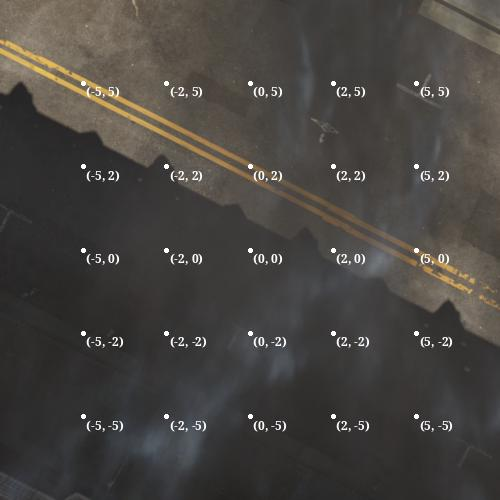
\includegraphics[width=0.5\linewidth]{images/GPT4o-CityNew-FS2/31_4.jpg}
    \end{center}
    
\gptspeaks: \( < \)Reasoning\( > \)The object is now clearly visible and I am centered directly above it at an altitude of 7 meters, which is below the required 10 meters. I have found the object.\( < \)/Reasoning\( > \)
\( < \)Action\( > \)FOUND\( < \)/Action\( > \)
\end{drama}
\subsubsection{Example}

    \begin{itemize}[noitemsep,topsep=0pt]
      \item Starting position: (4.0, 28.0, 109.0)
      \item End position: (-2.0, 2.0, 8.0) 
      \item Euclidean distance from the object: 8.48528137423857
      \item Object can be seen: True
      \item Success: True
      \item Object type: crowd
      
    \end{itemize}
    

    \begin{center}
    \includegraphics[width=0.7\linewidth]{images/GPT4o-CityNew-FS2/46.pdf}
    \end{center}
    

    \begin{center}
    \includegraphics[width=0.7\linewidth]{images/GPT4o-CityNew-FS2/46_sit_awareness.pdf}
    \end{center}
    

    \begin{drama}
    \Character{Benchmark}{re}
    \Character{GPT-4o}{gpt}
    
\respeaks: \( < \)Context\( > \)
    You are in command of a UAV, tasked with finding crowd.
\( < \)/Context\( > \) \texttt{(REST OF THE PROMPT)}
\respeaks: The object you're looking for is similar to this. This is NOT the drone's current view.
\StageDir{\re{} presents \gpt{} with a relevant image}

    \begin{center}
    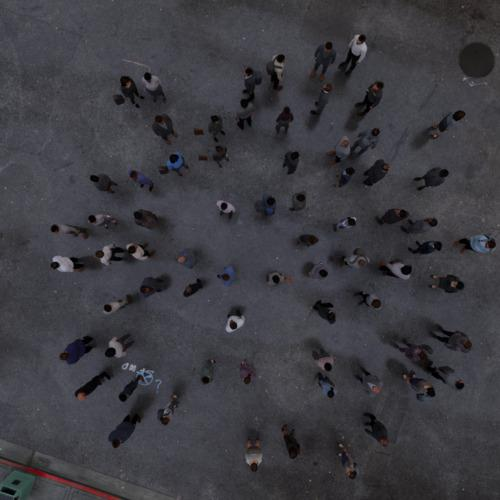
\includegraphics[width=0.5\linewidth]{images/GPT4o-CityNew-FS2/46_0.jpg}
    \end{center}
    
\respeaks: Your current altitude is 109 meters above ground level.
\StageDir{\re{} presents \gpt{} with a relevant image}

    \begin{center}
    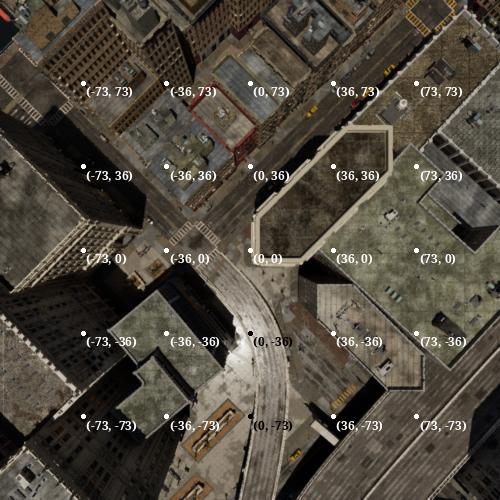
\includegraphics[width=0.5\linewidth]{images/GPT4o-CityNew-FS2/46_1.jpg}
    \end{center}
    
\gptspeaks: \( < \)Reasoning\( > \)The objective is to find the crowd. I will start by moving towards the center of the map to get a better view. The position (0, 0) is a good starting point for broad visibility.\( < \)/Reasoning\( > \)
\( < \)Action\( > \)(0, 0, 0)\( < \)/Action\( > \)
\respeaks: Your current altitude is 109 meters above ground level.
\StageDir{\re{} presents \gpt{} with a relevant image}

    \begin{center}
    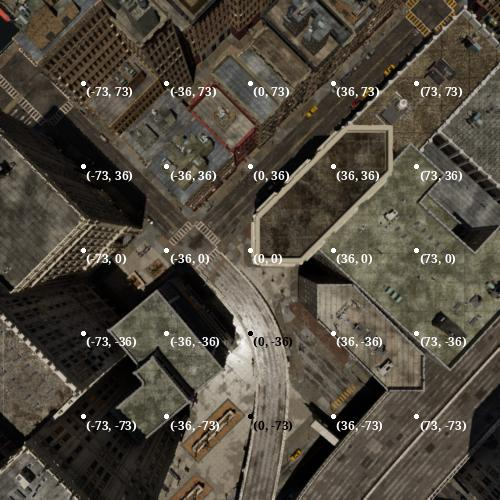
\includegraphics[width=0.5\linewidth]{images/GPT4o-CityNew-FS2/46_2.jpg}
    \end{center}
    
\gptspeaks: \( < \)Reasoning\( > \)I'm currently at the center. I need to lower the altitude to get a clearer view and check for the crowd. I'll descend by 30 meters to improve visibility.\( < \)/Reasoning\( > \)
\( < \)Action\( > \)(0, 0, -30)\( < \)/Action\( > \)
\respeaks: Your current altitude is 79 meters above ground level.
\StageDir{\re{} presents \gpt{} with a relevant image}

    \begin{center}
    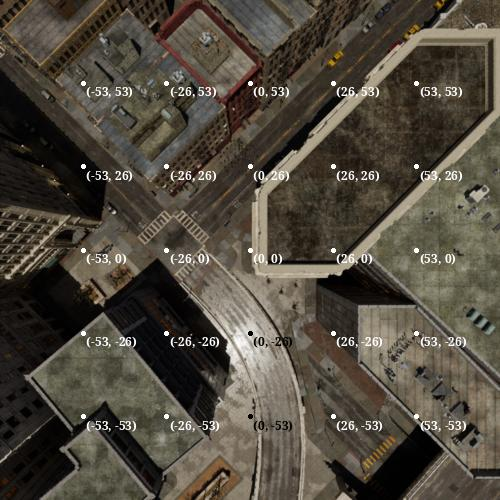
\includegraphics[width=0.5\linewidth]{images/GPT4o-CityNew-FS2/46_3.jpg}
    \end{center}
    
\gptspeaks: \( < \)Reasoning\( > \)I'm reducing altitude further to enhance visibility and check for the crowd. Descending by another 30 meters should help in identifying the object more clearly.\( < \)/Reasoning\( > \)
\( < \)Action\( > \)(0, 0, -30)\( < \)/Action\( > \)
\respeaks: Your current altitude is 49 meters above ground level.
\StageDir{\re{} presents \gpt{} with a relevant image}

    \begin{center}
    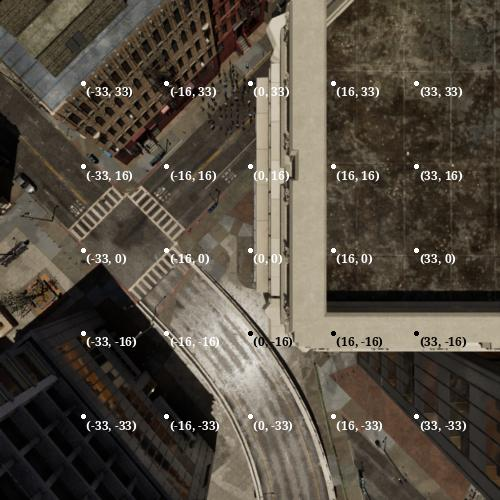
\includegraphics[width=0.5\linewidth]{images/GPT4o-CityNew-FS2/46_4.jpg}
    \end{center}
    
\gptspeaks: \( < \)Reasoning\( > \)I've spotted a group of people at (-16, 33). I will move towards that location and descend to get closer to confirm if it matches the objective. This will help center the drone on the crowd and ensure I'm below 10 meters above them.\( < \)/Reasoning\( > \)
\( < \)Action\( > \)(-16, 33, -40)\( < \)/Action\( > \)
\respeaks: Emergency stop; you've flown too close to something and would have hit it.
\respeaks: Your current altitude is 17 meters above ground level.
\StageDir{\re{} presents \gpt{} with a relevant image}

    \begin{center}
    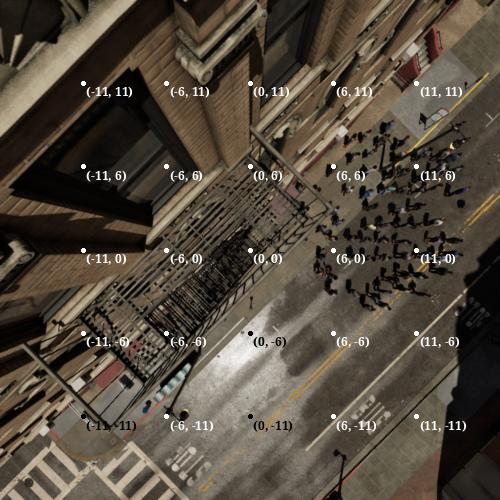
\includegraphics[width=0.5\linewidth]{images/GPT4o-CityNew-FS2/46_5.jpg}
    \end{center}
    
\gptspeaks: \( < \)Reasoning\( > \)The crowd is visible and centered in the field of view at (6, 0). I will descend a bit more to ensure I'm below 10 meters above ground level, which is necessary to confirm the find.\( < \)/Reasoning\( > \)
\( < \)Action\( > \)(6, 0, -9)\( < \)/Action\( > \)
\respeaks: Your current altitude is 8 meters above ground level.
\StageDir{\re{} presents \gpt{} with a relevant image}

    \begin{center}
    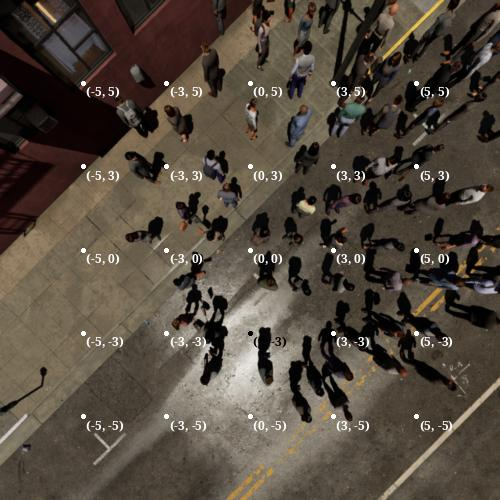
\includegraphics[width=0.5\linewidth]{images/GPT4o-CityNew-FS2/46_6.jpg}
    \end{center}
    
\gptspeaks: \( < \)Reasoning\( > \)The crowd is centered in the view, and I am at an appropriate altitude of 8 meters, which is within the required distance. I can confirm the find.\( < \)/Reasoning\( > \)
\( < \)Action\( > \)FOUND\( < \)/Action\( > \)
\end{drama}
